% \iffalse meta-comment
%
% This is file `mcmthesis.dtx'.
%
% Copyright (C)
%     2010 -- 2015 by Zhaoli Wang
%     2014 -- 2016 by Liam Huang
% -----------------------------------
% This work may be distributed and/or modified under the
% conditions of the LaTeX Project Public License, either version 1.3
% of this license or (at your option) any later version.
% The latest version of this license is in
%   http://www.latex-project.org/lppl.txt
% and version 1.3 or later is part of all distributions of LaTeX
% version 2005/12/01 or later.
%
% This work has the LPPL maintenance status `maintained'.
%
% The Current Maintainer of this work is Liam Huang.
%
%<*internal>
\begingroup
  \def\LaTeXeName{LaTeX2e}
\expandafter\endgroup\ifx\LaTeXeName\fmtname\else
\csname fi\endcsname
%</internal>
%<*install>
\input docstrip.tex
\keepsilent
\preamble

-----------------------------------

This is a generated file.

Copyright (C)
    2010 -- 2015 by Zhaoli Wang
    2014 -- 2016 by Liam Huang

This work may be distributed and/or modified under the
conditions of the LaTeX Project Public License, either version 1.3
of this license or (at your option) any later version.
The latest version of this license is in
  http://www.latex-project.org/lppl.txt
and version 1.3 or later is part of all distributions of LaTeX
version 2005/12/01 or later.

This work has the LPPL maintenance status `maintained'.

The Current Maintainer of this work is Liam Huang.

\endpreamble
\postamble

This work consists of these files \jobname.dtx,
                                  figures/ and
                                  code/,
and the derived files             \jobname.cls,
                                  \jobname-demo.tex,
                                  README,
                                  LICENSE,
                                  \jobname.pdf and
                                  \jobname-demo.pdf.
\endpostamble

\generate{%
  \usedir{tex/latex/\jobname}%
  \file{\jobname.cls}{\from{\jobname.dtx}{class}}%
  \usedir{doc/latex/\jobname}%
  \file{\jobname-demo.tex}{\from{\jobname.dtx}{demo}}%
  \nopreamble\nopostamble
  \file{README.tex}{\from{\jobname.dtx}{readme}}%
  \file{LICENSE.tex}{\from{\jobname.dtx}{license}}%
}
\obeyspaces
\Msg{*************************************************************}
\Msg{*                                                           *}
\Msg{* To finish the installation you have to                    *}
\Msg{*                                                           *}
\Msg{* produce the user manual run the file \jobname.dtx        *}
\Msg{* through XeLaTeX,                                          *}
\Msg{*                                                           *}
\Msg{* produce the demo file run the file \jobname-demo.tex     *}
\Msg{* through XeLaTeX,                                          *}
\Msg{*                                                           *}
\Msg{* move the following file into a directory searched         *}
\Msg{*    by TeX:                                                *}
\Msg{*                                                           *}
\Msg{*   \jobname.cls to TEXMF/tex/latex/mcmthesis/,            *}
\Msg{*   \jobname.dtx to TEXMF/source/latex/mcmthesis/,         *}
\Msg{*   other files   to TEXMF/doc/latex/mcmthesis/,            *}
\Msg{*                                                           *}
\Msg{* and then run texhash.                                     *}
\Msg{*                                                           *}
\Msg{* Happy TeXing!                                             *}
\Msg{*************************************************************}
\endbatchfile
%</install>
%<*internal>
\fi
%</internal>
%<*driver>
\ProvidesFile{mcmthesis.dtx}
  [2016/01/29 v6.2 The Thesis Template Designed For MCM/ICM]
\documentclass{ltxdoc}
\EnableCrossrefs
\CodelineIndex
\RecordChanges
\usepackage[UTF8, fntef, hyperref]{ctexcap}
\usepackage{hologo}
\usepackage{xcolor}
\usepackage{tabu}
\usepackage{longtable}
\usepackage{booktabs}
\usepackage{listings}
\usepackage{multirow}
\usepackage{amsmath}
\definecolor{grey}{rgb}{0.8,0.8,0.8}
\definecolor{darkgreen}{rgb}{0,0.3,0}
\definecolor{darkblue}{rgb}{0,0,0.3}
\lstset{
  language=[LaTeX]TeX,
% style
  frame=lines,%
  basicstyle={\footnotesize\ttfamily},%
  keywordstyle=\color{darkblue}\bfseries,%
  identifierstyle=,%
  commentstyle=\color{darkgreen},%\itshape,%
  stringstyle=\color{black}%
}
\AtBeginDocument{\hypersetup{colorlinks=true}}
\newcommand{\pkg}[1]{\textsf{#1}}
\newcommand{\env}[1]{\textsf{#1}}
\newcommand{\cntr}[1]{\textsf{#1}}
\newcommand{\XeLaTeX}{\hologo{XeLaTeX}}
\newcommand{\mem}[1]{\textcolor{blue}{\kaishu #1}}
\newcommand{\file}[1]{\textsf{#1}}
\newcommand{\path}[1]{\textsf{#1}}
\newcommand{\mopt}{\textsf}
\begin{document}
  \DocInput{\jobname.dtx}
\end{document}
%</driver>
% \fi
%
% \CheckSum{429}
%
% \CharacterTable
%  {Upper-case    \A\B\C\D\E\F\G\H\I\J\K\L\M\N\O\P\Q\R\S\T\U\V\W\X\Y\Z
%   Lower-case    \a\b\c\d\e\f\g\h\i\j\k\l\m\n\o\p\q\r\s\t\u\v\w\x\y\z
%   Digits        \0\1\2\3\4\5\6\7\8\9
%   Exclamation   \!     Double quote  \"     Hash (number) \#
%   Dollar        \$     Percent       \%     Ampersand     \&
%   Acute accent  \'     Left paren    \(     Right paren   \)
%   Asterisk      \*     Plus          \+     Comma         \,
%   Minus         \-     Point         \.     Solidus       \/
%   Colon         \:     Semicolon     \;     Less than     \<
%   Equals        \=     Greater than  \>     Question mark \?
%   Commercial at \@     Left bracket  \[     Backslash     \\
%   Right bracket \]     Circumflex    \^     Underscore    \_
%   Grave accent  \`     Left brace    \{     Vertical bar  \|
%   Right brace   \}     Tilde         \~}
%
% \changes{v1.0}{2013/05/12}{首次公开。}
%
% \GetFileInfo{\jobname.dtx}
%
% \DoNotIndex{\test}
%
% \title{\hypertarget{Chinese}{%
%   \textsf{\jobname} 文档类 \fileversion
%     \thanks{这份文档是 \textsf{\jobname}~\fileversion
%   的说明文档,更新日期 \filedate。}}%
%   \makebox[0pt][l]{\hspace{1.5cm}\hyperlink{English}%
%     {\large$ \to $ English Version}}
% }
% \author{王昭礼 \\ \texttt{343083553@qq.com}\and 黄晨成 \\ \texttt{liamhuang0205+\jobname@gmail.com}}
% \date{\filedate}
%
% \maketitle
%
% \begin{abstract}
%   这份模板是美国大学生数学建模竞赛(MCM/ICM)的论文模板。模板遵循赛事官方的要求,设置了
%   页眉页脚、字体和摘要页等内容。本文档对模板的使用做出了说明。
% \end{abstract}
%
% \section{模板介绍}
%
% 这份模板最早由王昭礼设计,并在往年参赛者的建议下不断改进。2014 年年初,黄晨成接手模板,
% 用 key-value 语法重构了文档选项,并修复了一些 bug。2015 年年初,黄晨成将模板使用
% \pkg{DocStrip} 的语法重构,并上传至 CTAN。
%
% 详细的使用说明,可以参考\href{http://liam0205.me/2016/01/27/how-to-use-mcmthesis/}{这里}。
%
% \section{手工安装说明}
%
% \subsection{下载}
%
% 你可以到项目主页下载模板的最新版本。除去项目主页之外,不再维护任何镜像。
%
% \begin{description}
%   \item [CTAN] \url{http://www.ctan.org/pkg/mcmthesis}
%   \item [GitHub] \url{https://github.com/Liam0205/mcmthesis}
% \end{description}
%
% 此外,文档类也已上传至 CTAN,你可以在 \TeX{} Live 等发行版的宏包管理器中下载。
%
% \subsection{安装}
%
% 我们以 \path{SOURCE} 代表你下载的源文件目录,在终端下执行以下命令。
% \iffalse
%<*internal>
% \fi
\begin{lstlisting}[language=bash]
cd SOURCE
xetex mcmthesis.dtx
xelatex mcmthesis.dtx
xelatex mcmthesis.dtx
xelatex mcmthesis-demo.tex
xelatex mcmthesis-demo.tex
\end{lstlisting}
% \iffalse
%</internal>
% \fi
%
% 你可以将生成的 \file{mcmthesis.cls} 拷贝至 \path{TEXMF/tex/latex/mcmthesis/}
% 目录,将 \file{mcmthesis.dtx} 拷贝至
% \path{TEXMF/source/latex/mcmthesis/},将 \file{mcmthesis.pdf}、
% \file{mcmthesis-demo.tex}、\file{mcmthesis-demo.pdf}、\file{figures/}
% 和 \file{code/} 拷贝至 \path{TEXMF/doc/latex/mcmthesis/},然后在终端
% 执行 \verb|texhash|;也可以将 \file{mcmthesis.cls} 放在当前目录直接使用。
%
% 生成的 \file{mcmthesis-demo.tex} 是一个示例文件,你可以参照这个文件来构建你的论文;
% 也可以直接修改这个文件。
%
% \section{使用说明}
% \subsection{依赖}
% \pkg{mcmthesis} 依赖于以下宏包,这些宏包在常见的 \TeX{} 发行版中都已包含,
% 在安装使用之前,请确认你的 \TeX{} 发行版中正确安装了这些宏包。
% \begin{longtabu}to 0.9\linewidth{*4{X[cm]}}
%   \toprule
%   \pkg{xkeyval} & \pkg{etoolbox} & \pkg{fancyhdr} & \pkg{fancybox} \\
%   \pkg{ifthen} & \pkg{lastpage} & \pkg{listings} & \pkg{appendix} \\
%   \pkg{amsmath} & \pkg{amssymb} & \pkg{amsfonts} & \pkg{amsbsy} \\
%   \pkg{bm} & \pkg{mathrsfs} & \pkg{latexsym} & \pkg{paralist} \\
%   \pkg{longtable} & \pkg{multirow} & \pkg{hhline} & \pkg{tabularx} \\
%   \pkg{ctex} & \pkg{xeCJK} & \pkg{CJK} & \pkg{xCJK2uni}\\
%   \pkg{tabu} & \pkg{environ} & \pkg{longtable} & \pkg{hologo}\\
%   \pkg{array} & \pkg{flafter} & \pkg{pifont} & \pkg{calc} \\
%   \pkg{colortbl} & \pkg{booktabs} & \pkg{geometry} & \pkg{fontenc}\\
%   \pkg{berasans} & \pkg{hyperref} & \pkg{ifpdf} & \pkg{ifxetex}\\
%   \pkg{graphicx} & \pkg{epstopdf} & \pkg{bmpsize} & \pkg{xcolor}\\
%   \pkg{longtable} & \pkg{tabu} & \pkg{hologo} & \pkg{palatino}\\
%   \bottomrule
% \end{longtabu}
% 如果你尚未安装这些宏包,可以启动你的 \TeX{} 发行版的宏包管理器
% 来安装;或者到 \url{http://www.ctan.org} 上搜索下载并安装。
%
% \subsection{选项}
% \pkg{mcmthesis} 定义了一些选项,用来控制模板的行为。
% 你可以在载入文档类的时候指定这些选项的值,例如
% \iffalse
%<*internal>
% \fi
\begin{lstlisting}[language={[LaTeX]TeX}]
\documentclass[tcn = 12345, problem = B, titlepage = false]{mcmthesis}
\end{lstlisting}
% \iffalse
%</internal>
% \fi
%\DescribeMacro{\mcmsetup}你也可以使用 \cs{mcmsetup}^^A
% \marg{key-value 列表} 来指定这些值,例如
% \iffalse
%<*internal>
% \fi
\begin{lstlisting}[language={[LaTeX]TeX}]
\documentclass{mcmthesis}
\mcmsetup{tcn = 12345, problem = B, titlepage = false}
\end{lstlisting}
% \iffalse
%</internal>
% \fi
% 两种做法效果等同。
%
% 当前,\pkg{mcmthesis} 有八个选项:
% \begin{description}
%   \item [CTeX] 兼容选项,默认关闭。当使用 2.9.2.164 版本的 CTeX 套装时请打开。
%   \item [tcn] 队伍控制号码,接受一个字符串作为值;输入的值将显示在摘要页上和
%     每一页的页眉上;默认为 \texttt{0000}。
%   \item [problem] 选题,接受一个字符串作为值;输入的值将显示在摘要页上;
%     默认为 \texttt{A}。
%   \item [sheet] 布尔值;为真时将输出摘要页,否则不输出;默认为 \texttt{true}。
%   \item [titleinsheet] 布尔值;为真时将在摘要页输出标题,否则不输出;
%     默认为 \texttt{false}。
%   \item [keywordsinsheet] 布尔值;为真时将在摘要页输出关键字,否则不输出;
%     默认为 \texttt{false}。
%   \item [titlepage] 布尔值;为真时将输出标题页,否则不输出;默认为 \texttt{true}。
%   \item [abstract] 布尔值;为真时将在标题页输出摘要和关键词,否则不输出;默认值为
%     \texttt{true}。
% \end{description}
%
% 注意,\texttt{titleinsheet} 和 \texttt{keywordsinsheet} 的效果受 \texttt{sheet}
% 的影响。若 \texttt{sheet = false},则不论前二者的真假,均不会在摘要页上输出标题和/或
% 关键字。另一方面,若 \texttt{sheet = true},则摘要部分总是会出现在摘要页。
% \texttt{abstract} 与 \texttt{titlepage} 选项的关系于前述类似。
%
% \subsection{题号}
%
% \DescribeMacro{\problem}除了使用 \cs{mcmsetup} 来指定题号,你还可以使用
% \cs{problem}\marg{题号} 命令来选择题号。后一种方式是为了兼容而提供的,不推荐
% 使用。
%
% \subsection{环境}
%
% \DescribeEnv{abstract}\DescribeEnv{keywords}
% \pkg{mcmthesis} 重新定义了 \env{abstract} 环境,并且
% 定义了 \env{keywords} 环境。需要注意的是,他们的行为和
% \LaTeX{} 标准的 \cs{title} 命令类似——在使用的时候,只是记录内容,而并不输出内容;
% 内容的实际输出要等到 \cs{maketitle} 命令。
%
% \subsection{摘要页头部设置}
% \DescribeMacro{\headset}MCM/ICM 的主办方经常变动摘要页头部的年份及赛事名称说明的格式,可谓岁岁年年各不同。因此,模板很难保证这部分的格式与当年的要求完全一致,故而给出一个易于修改的接口。例如:
% \iffalse
%<*internal>
% \fi
\begin{lstlisting}[language={[LaTeX]TeX}]
\renewcommand{\headset}{{\Large\the\year}\\MCM/ICM\\Summary Sheet}
\end{lstlisting}
% \iffalse
%</internal>
% \fi
% 将会输出:
% \begin{trivlist}\item
% \newcommand{\headset}{{\Large\the\year}\\MCM/ICM\\Summary Sheet}
% \begin{center}
%   \textbf{\headset}
% \end{center}
% \end{trivlist}
%
% \subsection{编译方式}
%
% 模板支持多种编译方式:
% \begin{itemize}
%   \item \XeLaTeX \textbf{这是推荐的方式};
%   \item pdf\LaTeX;
%   \item \LaTeX{} + DVIPDFMx。
% \end{itemize}
%
% \subsection{中文支持}
%
% 由于 MCM/ICM 要求以英文写作,所以模板没有内建的中文支持。如果你在文章中需要使用个别中文
% 字符,可以自行使用合适中文支持方式。例如,使用 CTeX 宏集:
%
% \iffalse
%<*internal>
% \fi
\begin{lstlisting}[language={[LaTeX]TeX}]
\usepackage[UTF8, nocap]{ctex}
\end{lstlisting}
% \iffalse
%</internal>
% \fi
%
% \section{版本历史}
% \begin{description}
%   \item [5.1.0a] 首次上传到 CTAN。
%   \item [5.1.0b] 修复 \textsf{CheckSum} 和一些拼写错误。
%   \item [5.1.0c] 新增 \mopt{titleinsheet} 等选项。
%   \item [5.1.0d] 修改 \mopt{problem} 的定义方式,定义
%     \cs{mcmsetup}\marg{key-val 列表} 以修改选项,
%     调高了摘要页表格的位置,修复摘要页和标题页页码的问题,
%     修复标题、摘要和关键字过长时分行、分页的问题。
%   \item [5.1.0e] 重新定义摘要页顶部的表格,以符合赛事主办方 COMAP 的最新版的
%     摘要页。
%   \item [5.1.0f] 取消 TCN 和选题的红色标记。
%   \item [6.0] 微调输出格式,新增选项 CTeX 以兼容 2.9.2.164 版本的 CTeX 套装。
%   \item [6.1] 修复问题。
%   \item [6.2] 可定制的 headset.
% \end{description}
%
% \title{\hypertarget{English}{%
%   The \textsf{\jobname} class \fileversion\thanks{This Document
%   corresponds to \textsf{\jobname}~\fileversion, dated \filedate.}}%
%   \makebox[0pt][l]{\hspace{1.5cm}\hyperlink{Chinese}{\large$ \to $ 中文版}}
% }
% \author{Zhaoli Wang \\ \texttt{\texttt{343083553@qq.com}}\and Liam Huang \\ \texttt{liamhuang0205+\jobname@gmail.com}}
% \date{\filedate}
%
% \maketitle
%
% \renewcommand{\abstractname}{Abstract}
% \begin{abstract}
%   This template is designed for MCM/ICM. The template configured fonts,
%   header and footer and summary sheet style, accroding to the requirements
%   of COMAP. This document desicribes the template.
% \end{abstract}
%
% \section{Introduction}
%
% This template was designed by Zhaoli Wang first, and was improved by him
% following the suggestions from contest takers. In the beginning of the year
% 2014, Liam Huang redesigned it, by using key-value syntax, and fixed known
% bugs. Liam reimplemented it at the begining of the year 2015,
% by \pkg{DocStrip}, and uploaded it to CTAN.
%
% \section{Installation Guide}
%
% \subsection{Download}
%
% You could find the latest version of this template at the project
% homepage. We will
% not maintain any other mirror.
%
% \begin{description}
%   \item [CTAN] \url{http://www.ctan.org/pkg/mcmthesis}
%   \item [GitHub] \url{https://github.com/Liam0205/mcmthesis}
% \end{description}
%
% Moreover, this template had been uploaded to CTAN, so that it could
% be managed by the package manager of your distribution, such as \TeX\ Live.
%
% \subsection{Installation}
%
% We denote \path{SOURCE} as the folder, who contains the file you've
% just downloaded. Execute these command in the terminal.
% \iffalse
%<*internal>
% \fi
\begin{lstlisting}[language=bash]
cd SOURCE
xetex mcmthesis.dtx
xelatex mcmthesis.dtx
xelatex mcmthesis.dtx
xelatex mcmthesis-demo.tex
xelatex mcmthesis-demo.tex
\end{lstlisting}
% \iffalse
%</internal>
% \fi
%
% To finish the installation, you could copy \file{mcmthesis.cls} to
% \path{TEXMF/tex/latex/mcmthesis/}, copy \file{mcmthesis.dtx}
% to \path{TEXMF/source/latex/mcmthesis/},
% copy \file{mcmthesis.pdf}, \file{mcmthesis-demo.tex},
% \file{mcmthesis-demo.pdf}, \file{figures/} and \file{code/} to
% \path{TEXMF/doc/latex/mcmthesis/}, and then run \verb|texhash| in your
% terminal; you could also put \file{mcmthesis.cls} in the same folder of
% the master file.
%
% \file{mcmthesis-demo.tex} is a generated demo file, you could write the
% manuscript of you paper by mimicing this file; you may also modify this
% file to build your paper.
%
% \section{Usage}
% \subsection{Dependence}
% The \pkg{mcmthesis} class depends on the following pakcages.
% These packages has been installed in common \TeX{} distribution.
% Before installation, please make sure that you have installed these
% packages correctly.
% \begin{longtabu}to 0.9\linewidth{*4{X[cm]}}
%   \toprule
%   \pkg{xkeyval} & \pkg{etoolbox} & \pkg{fancyhdr} & \pkg{fancybox} \\
%   \pkg{ifthen} & \pkg{lastpage} & \pkg{listings} & \pkg{appendix} \\
%   \pkg{amsmath} & \pkg{amssymb} & \pkg{amsfonts} & \pkg{amsbsy} \\
%   \pkg{bm} & \pkg{mathrsfs} & \pkg{latexsym} & \pkg{paralist} \\
%   \pkg{longtable} & \pkg{multirow} & \pkg{hhline} & \pkg{tabularx} \\
%   \pkg{ctex} & \pkg{xeCJK} & \pkg{CJK} & \pkg{xCJK2uni}\\
%   \pkg{tabu} & \pkg{environ} & \pkg{longtable} & \pkg{hologo}\\
%   \pkg{array} & \pkg{flafter} & \pkg{pifont} & \pkg{calc} \\
%   \pkg{colortbl} & \pkg{booktabs} & \pkg{geometry} & \pkg{fontenc}\\
%   \pkg{berasans} & \pkg{hyperref} & \pkg{ifpdf} & \pkg{ifxetex}\\
%   \pkg{graphicx} & \pkg{epstopdf} & \pkg{bmpsize} & \pkg{xcolor}\\
%   \pkg{longtable} & \pkg{tabu} & \pkg{hologo} & \pkg{palatino}\\
%   \bottomrule
% \end{longtabu}
% If you haven't install these packages, you could execute the package
% manager of your distribution and install them; you could also download
% them from \url{http://www.ctan.org}.
%
% \subsection{Options}
% \pkg{mcmthesis} defined serval options to control the behaviour of
% the template. You could specify these options while loading the class.
% \iffalse
%<*internal>
% \fi
\begin{lstlisting}[language={[LaTeX]TeX}]
\documentclass[tcn = 12345, problem = B, titlepage = false]{mcmthesis}
\end{lstlisting}
% \iffalse
%</internal>
% \fi
%\DescribeMacro{\mcmsetup}You may also use the command \cs{mcmsetup}^^A
% \marg{key-value list} to specify them.
% \iffalse
%<*internal>
% \fi
\begin{lstlisting}[language={[LaTeX]TeX}]
\documentclass{mcmthesis}
\mcmsetup{tcn = 12345, problem = B, titlepage = false}
\end{lstlisting}
% \iffalse
%</internal>
% \fi
% The two methods share the same effect.
%
% \pkg{mcmthesis} has seven options.
% \begin{description}
%   \item [tcn] The team control number, recieves a string as value;
%     this value will be displayed on summary sheet and every page's header.
%     The default value is \texttt{0000}.
%   \item [problem] The question, recieves a string as value;
%     this value will be displayed on summary sheet.
%     The default value is \texttt{A}.
%   \item [sheet] Bool, true to print the summary sheet, default
%     is \texttt{true}.
%   \item [titleinsheet] Bool, true to print the title in the summary sheet,
%     default is \texttt{false}.
%   \item [keywordsinsheet] Bool, true to print keywords in the summary sheet,
%     default is \texttt{false}.
%   \item [titlepage] Bool, true to print the titlepage,
%     default is \texttt{true}.
%   \item [abstract] Bool, true to print the abstract on the titlepage,
%     default is \texttt{true}.
% \end{description}
%
% Note that the effect of \texttt{titleinsheet} and \texttt{keywordsinsheet}
% are under the control of the option \texttt{sheet}, that is, if
% \texttt{sheet} is set to \texttt{false}, title and/or keywords will not be
% printed on the summary sheet, whatever the value of these two options are.
% On the other hand, the abstract will always be printed on the summary sheet,
% if the \texttt{sheet} is set to \texttt{true}. The relationship between
% \texttt{abstract} and \texttt{titlepage} is similar to that just mentioned.
%
% \subsection{Question}
%
% \DescribeMacro{\problem}Besides using \cs{mcmsetup} to choose question,
% you could also use \cs{problem}\marg{Question} to do this.
% However, the later one is here just because of backward compatibility,
% and is not recommended any longer.
%
% \subsection{Environment}
%
% \DescribeEnv{abstract}\DescribeEnv{keywords}
% \pkg{mcmthesis} redefined the \env{abstract} environment, and defined a
% new environment named \env{keywords}. Note that these two environments
% behave like the standard \cs{title} --- they will not print any contents
% to the PDF file when they are used but just record them; the output task
% belongs to \cs{maketitle}.
%
% \subsection{The headset of the Summary Sheet}
% \DescribeMacro{\headset}Due to the frequent change of the headset's style of the Summary Sheet from the host of MCM/ICM, it's difficult for me to keep in with. Hence, a easy-to-modified interfaced is designed. Let's see an succinct example:
% \iffalse
%<*internal>
% \fi
\begin{lstlisting}[language={[LaTeX]TeX}]
\renewcommand{\headset}{{\Large\the\year}\\MCM/ICM\\Summary Sheet}
\end{lstlisting}
% \iffalse
%</internal>
% \fi
% while the output is:
% \begin{trivlist}\item
% \newcommand{\headset}{{\Large\the\year}\\MCM/ICM\\Summary Sheet}
% \begin{center}
%   \textbf{\headset}
% \end{center}
% \end{trivlist}
%
% \subsection{Compilation Workflow}
%
% The template supports various kinds of compilation workflow:
% \begin{itemize}
%   \item \XeLaTeX\ (\textbf{recommend});
%   \item pdf\LaTeX;
%   \item \LaTeX{} + DVIPDFMx。
% \end{itemize}
%
%
% \section{History}
% \begin{description}
%   \item [5.1.0a] First release to CTAN.
%   \item [5.1.0b] Fix the bug of \textsf{CheckSum} and typos.
%   \item [5.1.0c] Import options, such as \mopt{titleinsheet}.
%   \item [5.1.0d] Change the way to define \mopt{problem}, create
%     \cs{mcmsetup}\marg{key-val list} to modify the option, slightly lift
%     the table on the summary sheet, fix the
%     bug of page number and fix the bug of title, abstract and keywords.
%   \item [5.1.0e] Redefine the table at the top of the summary sheet to
%     match the latest summary sheet from COMAP, the maker of the contest.
%   \item [5.1.0f] Cancle the red emphasizing of tcn and problem mark in the
%     table at the topo of the summary sheet.
%   \item [6.0] Change the output style slightly.
%   \item [6.1] Bugfix.
%   \item [6.2] Making headset of the Summary Sheet modifible.
% \end{description}
%
% \StopEventually{}
% \section{The Implementation}
% \subsection{Basic Information}
%    \begin{macrocode}
%<*class>
\NeedsTeXFormat{LaTeX2e}[1999/12/01]
\ProvidesClass{mcmthesis}
  [2016/01/29 v6.2 The Thesis Template Designed For MCM/ICM]
\typeout{The Thesis Template Designed For MCM/ICM}
\def\MCMversion{v6.2}
%    \end{macrocode}
% \subsection{Options}
%
% Loading \pkg{xkeyval} and \pkg{etoolbox} to handle key-value options.
%    \begin{macrocode}
\RequirePackage{xkeyval}
\RequirePackage{etoolbox}
%    \end{macrocode}
%
% Declaring options.
%    \begin{macrocode}
\define@boolkey{MCM}[MCM@opt@]{CTeX}[false]{}
\define@boolkey{MCM}[MCM@opt@]{titlepage}[true]{}
\define@boolkey{MCM}[MCM@opt@]{abstract}[true]{}
\define@boolkey{MCM}[MCM@opt@]{sheet}[true]{}
\define@boolkey{MCM}[MCM@opt@]{titleinsheet}[false]{}
\define@boolkey{MCM}[MCM@opt@]{keywordsinsheet}[false]{}
\define@cmdkeys{MCM}[MCM@opt@]{tcn,problem}
\define@key{MCM}{tcn}[0000]{\gdef\MCM@opt@tcn{#1}}
\define@key{MCM}{problem}[A]{\gdef\MCM@opt@problem{#1}}
\setkeys{MCM}{tcn=0000,problem=B}

\define@key{mcmthesis.cls}{tcn}[0000]{\gdef\MCM@opt@tcn{#1}}
\define@key{mcmthesis.cls}{problem}[A]{\gdef\MCM@opt@problem{#1}}
\define@boolkey{mcmthesis.cls}[MCM@opt@]{titlepage}{}
\define@boolkey{mcmthesis.cls}[MCM@opt@]{abstract}{}
\define@boolkey{mcmthesis.cls}[MCM@opt@]{sheet}{}
\define@boolkey{mcmthesis.cls}[MCM@opt@]{titleinsheet}{}
\define@boolkey{mcmthesis.cls}[MCM@opt@]{keywordsinsheet}{}
\MCM@opt@sheettrue
\MCM@opt@titlepagetrue
\MCM@opt@titleinsheetfalse
\MCM@opt@keywordsinsheetfalse
\MCM@opt@abstracttrue
%    \end{macrocode}
%
% \begin{macro}{\mcmsetup}
%
%    \begin{macrocode}
\newcommand{\mcmsetup}[1]{\setkeys{MCM}{#1}}
%    \end{macrocode}
% \end{macro}
%
% Processing options.
%    \begin{macrocode}
\ProcessOptionsX\relax
%    \end{macrocode}
%
% Loading document class.
%    \begin{macrocode}
\LoadClass[a4paper, 11pt]{article}
%    \end{macrocode}
%
% User interface.
%    \begin{macrocode}
\newcommand{\team}{Team \#\ \MCM@opt@tcn}
%    \end{macrocode}
% \subsection{Loading Packages}
%    \begin{macrocode}
\RequirePackage{fancyhdr, fancybox}
\RequirePackage{ifthen}
\RequirePackage{lastpage}
\RequirePackage{listings}
\RequirePackage[toc, page, title, titletoc, header]{appendix}
\RequirePackage{paralist}
\RequirePackage{amsthm, amsfonts}
\RequirePackage{amsmath, bm}
\RequirePackage{amssymb, mathrsfs}
\RequirePackage{latexsym}
\RequirePackage{longtable, multirow, hhline, tabularx, array}
\RequirePackage{flafter}
\RequirePackage{pifont, calc}
\RequirePackage{colortbl, booktabs}
\RequirePackage{geometry}
\RequirePackage[T1]{fontenc}
\RequirePackage[scaled]{berasans}
\RequirePackage{hyperref}
\RequirePackage{ifpdf, ifxetex}
\AtBeginDocument{
\ifMCM@opt@CTeX
\else
  \RequirePackage{environ}
\fi
}
%    \end{macrocode}
%
% Loading \pkg{graphicx} and its relations after checking drivers.
%    \begin{macrocode}
\ifpdf
  \RequirePackage{graphicx}
  \RequirePackage{epstopdf}
\else
  \ifxetex
    \RequirePackage{graphicx}
  \else
    \RequirePackage[dvipdfmx]{graphicx}
    \RequirePackage{bmpsize}
  \fi
\fi
\RequirePackage{xcolor}
%    \end{macrocode}
% \subsection{\pkg{hyperref} Settings}
%    \begin{macrocode}
\ifpdf
  \hypersetup{hidelinks}
\else
  \ifxetex
    \hypersetup{hidelinks}
  \else
    \hypersetup{dvipdfm, hidelinks}
  \fi
\fi
%    \end{macrocode}
% \subsection{Page Layout}
% Setting paper size and margin sep.
%    \begin{macrocode}
\geometry{a4paper, margin = 1.2in}
%    \end{macrocode}
%
% Making the footer and header.
%    \begin{macrocode}
\pagestyle{fancy}
\fancyhf{}
\lhead{\small\sffamily \team}
\rhead{\small\sffamily Page \thepage\ of \pageref{LastPage}}
%    \end{macrocode}
%
% Setting \cs{parskip}.
%    \begin{macrocode}
\setlength\parskip{.5\baselineskip}
%    \end{macrocode}
% \subsection{Redefining TOC}
%    \begin{macrocode}
\renewcommand\tableofcontents{%
    \centerline{\normalfont\Large\bfseries\sffamily\contentsname
        \@mkboth{%
           \MakeUppercase\contentsname}{\MakeUppercase\contentsname}}%
    \vskip 5ex%
    \@starttoc{toc}%
    }
%    \end{macrocode}
% \subsection{Mastering Floats, Figures and Tables}
% Setting counters. Here \cntr{totalnumber} is the maximum number of
% floats on a text page, \cntr{topnumber} is the maximum number of
% floats at top of a text page and \cntr{bottomnumber} is the maximum
% number of floats at bottom of a text page. Obviously, we have
% $ \text{\cntr{totalnumber}} = \text{\cntr{topnumber}} +
% \text{\cntr{bottomnumber}} $.
%    \begin{macrocode}
\setcounter{totalnumber}{4}
\setcounter{topnumber}{2}
\setcounter{bottomnumber}{2}
%    \end{macrocode}
%
% Setting float fractions.
%    \begin{macrocode}
\renewcommand{\textfraction}{0.15}
\renewcommand{\topfraction}{0.85}
\renewcommand{\bottomfraction}{0.65}
\renewcommand{\floatpagefraction}{0.60}
%    \end{macrocode}
%
% Setting caption names.
%    \begin{macrocode}
\renewcommand{\figurename}{Figure}
\renewcommand{\tablename}{Table}
%    \end{macrocode}
%
% Setting graphic paths.
%    \begin{macrocode}
\graphicspath{{./}{./img/}{./fig/}{./image/}{./figure/}{./picture/}
            {./imgs/}{./figs/}{./images/}{./figures/}{./pictures/}}
%    \end{macrocode}
% \subsection{Designing Sheets and their Relations}
% Redefining \cs{maketitle}, which will check if the control
% sheet and titlepage should be printed.
%    \begin{macrocode}
\def\maketitle{%
  \let\saved@thepage\thepage
  \let\thepage\relax
  \ifMCM@opt@sheet
  \makesheet
  \fi
  \newpage
  \ifMCM@opt@titlepage
    \MCM@maketitle
  \fi
  \newpage
  \let\thepage\saved@thepage
  \setcounter{page}{1}
  \pagestyle{fancy}
}
%    \end{macrocode}
%
% Making the \env{abstract} environment.
%    \begin{macrocode}
\def\abstractname{Abstract}
\def\sheetsummaryname{Summary}
\def\keywordsname{Keywords}
\AtBeginDocument{
\ifMCM@opt@CTeX
  \newbox\@abstract%
  \setbox\@abstract\hbox{}%
  \long\def\abstract{\bgroup\global\setbox\@abstract\vbox\bgroup\hsize\textwidth\leftskip1cm\rightskip1cm}%
  \def\endabstract{\egroup\egroup}
  \def\make@abstract{%
    \begin{center}
      \textbf{\abstractname}
    \end{center}
    \usebox\@abstract\par
  }
  \newbox\@sheetsummary%
  \setbox\@sheetsummary\hbox{}%
  \long\def\sheetsummary{\bgroup\global\setbox\@sheetsummary\vbox\bgroup\hsize\textwidth\leftskip1cm\rightskip1cm}%
  \def\endsheetsummary{\egroup\egroup}
  \def\make@sheetsummary{%
    \begin{center}
      \textbf{\sheetsummaryname}
    \end{center}
    \usebox\@sheetsummary\par
  }
  \newbox\@keywords
  \setbox\@keywords\hbox{}
  \def\keywords{\global\setbox\@keywords\vbox\bgroup\noindent\leftskip0cm}
  \def\endkeywords{\egroup}%
  \def\make@keywords{%
   \par\hskip.4cm\textbf{\keywordsname}: \usebox\@keywords\hfill\par
  }
\else
  \NewEnviron{sheetsummary}{\xdef\@sheetsummary{\expandonce\BODY}}
  \def\make@sheetsummary{%
    \begin{center}
      \textbf{\sheetsummaryname}
    \end{center}
    \@sheetsummary\par
  }
  \RenewEnviron{abstract}{\xdef\@abstract{\expandonce\BODY}}
  \def\make@abstract{%
    \begin{center}
      \textbf{\abstractname}
    \end{center}
    \@abstract\par
  }
  \NewEnviron{keywords}{\xdef\@keywords{\expandonce\BODY}}
  \def\make@keywords{%
    \par\noindent\textbf{\keywordsname}:
    \@keywords\par
  }
\fi
}
%    \end{macrocode}
%
% Making the \env{keywords} environment.
%    \begin{macrocode}
 

%    \end{macrocode}
%
% \begin{macro}{\headset}
%
%    \begin{macrocode}
\newcommand{\headset}{{\Large\the\year}\\MCM/ICM\\Summary Sheet}
%    \end{macrocode}
% \end{macro}
%
% Defining the \cs{makesheet}.
%    \begin{macrocode}
\newcommand{\problem}[1]{\mcmsetup{problem = #1}}
\def\makesheet{%
  \pagestyle{empty}%
  \null%
  \vspace*{-5pc}%
  \begin{center}
  \begingroup
  \setlength{\parindent}{0pt}
     \begin{minipage}{0.28\linewidth}
      For office use only\\[4pt]
      \makebox[0.15\linewidth][l]{T1}\rule[-2pt]{0.85\linewidth}{0.5pt}\\[4pt]
      \makebox[0.15\linewidth][l]{T2}\rule[-2pt]{0.85\linewidth}{0.5pt}\\[4pt]
      \makebox[0.15\linewidth][l]{T3}\rule[-2pt]{0.85\linewidth}{0.5pt}\\[4pt]
      \makebox[0.15\linewidth][l]{T4}\rule[-2pt]{0.85\linewidth}{0.5pt}
     \end{minipage}%
     \begin{minipage}{0.44\linewidth}
      \centering
      Team Control Number\\[0.7pc]
      {\Huge\textbf{\MCM@opt@tcn}}\\[1.8pc]
      Problem Chosen\\[0.7pc]
      {\huge\textbf{\MCM@opt@problem}}
     \end{minipage}%
     \begin{minipage}{0.28\linewidth}
      For office use only\\[4pt]
      \makebox[0.15\linewidth][l]{F1}\rule[-2pt]{0.85\linewidth}{0.5pt}\\[4pt]
      \makebox[0.15\linewidth][l]{F2}\rule[-2pt]{0.85\linewidth}{0.5pt}\\[4pt]
      \makebox[0.15\linewidth][l]{F3}\rule[-2pt]{0.85\linewidth}{0.5pt}\\[4pt]
      \makebox[0.15\linewidth][l]{F4}\rule[-2pt]{0.85\linewidth}{0.5pt}
     \end{minipage}\par
  \rule{\linewidth}{0.5pt}\par
  \textbf{\headset}%
  \par
  \endgroup
  \vskip 10pt%
  \ifMCM@opt@titleinsheet
    \normalfont \LARGE \@title \par
  \fi
  \end{center}
\ifMCM@opt@keywordsinsheet
  \make@sheetsummary%
  \make@keywords%
\else
  \make@sheetsummary%
\fi}
%    \end{macrocode}
%
% Defining the \cs{MCM@maketitle}
%    \begin{macrocode}
\newcommand{\MCM@maketitle}{%
  \begin{center}%
  \let \footnote \thanks
    {\LARGE \@title \par}%
    \vskip 1.5em%
    {\large
      \lineskip .5em%
      \begin{tabular}[t]{c}%
        \@author
      \end{tabular}\par}%
    \vskip 1em%
    {\large \@date}%
  \end{center}%
  \par
  \vskip 1.5em%
  \ifMCM@opt@abstract%
    \make@abstract
    \make@keywords
  \fi%
}
%    \end{macrocode}
% \subsection{Mathematics}
% Theorems.
%    \begin{macrocode}
\newtheorem{Theorem}{Theorem}[section]
\newtheorem{Lemma}[Theorem]{Lemma}
\newtheorem{Corollary}[Theorem]{Corollary}
\newtheorem{Proposition}[Theorem]{Proposition}
\newtheorem{Definition}[Theorem]{Definition}
\newtheorem{Example}[Theorem]{Example}
%    \end{macrocode}
%
% Other definitions.
%    \begin{macrocode}
\providecommand{\dif}{\mathop{}\!\mathrm{d}}
\providecommand{\me}{\mathrm{e}}
\providecommand{\mi}{\mathrm{i}}
%    \end{macrocode}
% \subsection{Listing Settings}
%    \begin{macrocode}
\definecolor{grey}{rgb}{0.8,0.8,0.8}
\definecolor{darkgreen}{rgb}{0,0.3,0}
\definecolor{darkblue}{rgb}{0,0,0.3}
\def\lstbasicfont{\fontfamily{pcr}\selectfont\footnotesize}
\lstset{%
% indexing
   % numbers=left,
   % numberstyle=\small,%
% character display
    showstringspaces=false,
    showspaces=false,%
    tabsize=4,%
% style
    frame=lines,%
    basicstyle={\footnotesize\lstbasicfont},%
    keywordstyle=\color{darkblue}\bfseries,%
    identifierstyle=,%
    commentstyle=\color{darkgreen},%\itshape,%
    stringstyle=\color{black}%
}
\lstloadlanguages{C,C++,Java,Matlab,Mathematica}
%    \end{macrocode}
%    \begin{macrocode}
%</class>
%<class>\endinput
%    \end{macrocode}
% \iffalse
%<*demo>
%!TEX program = xelatex
\documentclass{mcmthesis}
\mcmsetup{CTeX = false,   % 使用 CTeX 套装时,设置为 true
        tcn = 0000, problem = A,
        sheet = true, titleinsheet = true, keywordsinsheet = true,
        titlepage = true, abstract = true}
\usepackage{palatino}
\usepackage{lipsum}
\title{The \LaTeX{} Template for MCM Version \MCMversion}
\author{\small \href{http://www.latexstudio.net/}
  {
\includegraphics[width=7cm]{mcmthesis-logo}}}
\date{\today}

 %正文摘要和控制页摘要名字修改
\def\abstractname{Abstract}
\def\sheetsummaryname{Summary}

\begin{document}

 %控制页摘要内容
\begin{sheetsummary}
\lipsum[1]
\end{sheetsummary}

 %正文摘要内容
\begin{abstract}
\lipsum[1]
\end{abstract}

 %关键词
\begin{keywords}
keyword1; keyword2
\end{keywords}

\maketitle
 % Generate the Table of Contents, if it's needed.
 % \tableofcontents
 % \newpage
\section{Introduction}

\lipsum[2]
\begin{itemize}
\item minimizes the discomfort to the hands, or
\item maximizes the outgoing velocity of the ball.
\end{itemize}
We focus exclusively on the second definition.

\begin{itemize}
\item the initial velocity and rotation of the ball,
\item the initial velocity and rotation of the bat,
\item the relative position and orientation of the bat and ball, and
\item the force over time that the hitter hands applies on the handle.
\end{itemize}
\lipsum[3]
\begin{itemize}
\item the angular velocity of the bat,
\item the velocity of the ball, and
\item the position of impact along the bat.
\end{itemize}
\lipsum[4]
\emph{center of percussion} [Brody 1986], \lipsum[5]

\begin{Theorem} \label{thm:latex}
\LaTeX
\end{Theorem}
\begin{Lemma} \label{thm:tex}
\TeX .
\end{Lemma}
\begin{proof}
The proof of theorem.
\end{proof}

\subsection{Other Assumptions}
\lipsum[6]
\begin{itemize}
\item
\item
\item
\item
\end{itemize}

\lipsum[7]

\section{Analysis of the Problem}
\begin{figure}[h]
\small
\centering
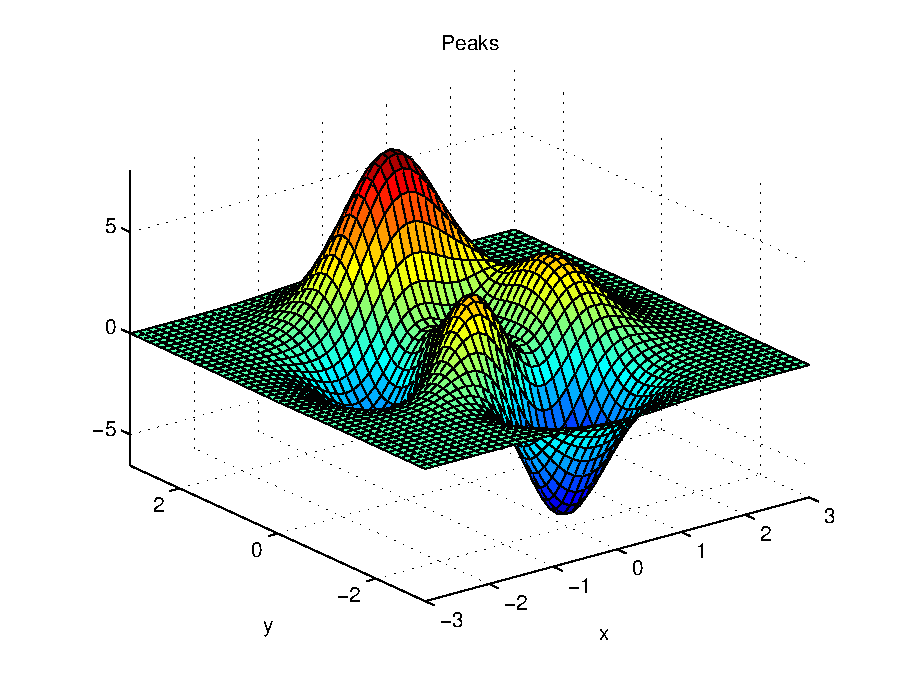
\includegraphics[width=12cm]{mcmthesis-aaa.eps}
\caption{aa} \label{fig:aa}
\end{figure}

\lipsum[8] \eqref{aa}
\begin{equation}
a^2 \label{aa}
\end{equation}


\[
  \begin{pmatrix}{*{20}c}
  {a_{11} } & {a_{12} } & {a_{13} }  \\
  {a_{21} } & {a_{22} } & {a_{23} }  \\
  {a_{31} } & {a_{32} } & {a_{33} }  \\
  \end{pmatrix}
  = \frac{{Opposite}}{{Hypotenuse}}\cos ^{ - 1} \theta \arcsin \theta
\]
\lipsum[9]

\[
  p_{j}=\begin{cases} 0,&\text{if $j$ is odd}\\
  r!\,(-1)^{j/2},&\text{if $j$ is even}
  \end{cases}
\]

\lipsum[10]

\[
  \arcsin \theta  =
  \mathop{{\int\!\!\!\!\!\int\!\!\!\!\!\int}\mkern-31.2mu
  \bigodot}\limits_\varphi
  {\mathop {\lim }\limits_{x \to \infty } \frac{{n!}}{{r!\left( {n - r}
  \right)!}}} \eqno (1)
\]

\section{Calculating and Simplifying the Model  }
\lipsum[11]

\section{The Model Results}
\lipsum[6]

\section{Validating the Model}
\lipsum[9]

\section{Conclusions}
\lipsum[6]

\section{A Summary}
\lipsum[6]

\section{Evaluate of the Mode}

\section{Strengths and weaknesses}
\lipsum[12]

\subsection{Strengths}
\begin{itemize}
\item \textbf{Applies widely}\\
This  system can be used for many types of airplanes, and it also
solves the interference during  the procedure of the boarding
airplane,as described above we can get to the  optimization
boarding time.We also know that all the service is automate.
\item \textbf{Improve the quality of the airport service}\\
Balancing the cost of the cost and the benefit, it will bring in
more convenient  for airport and passengers.It also saves many
human resources for the airline. \item \textbf{}
\end{itemize}

\begin{thebibliography}{99}
%\addcontentsline{toc}{section}{References}
\bibitem{1} D.~E. KNUTH   The \TeX{}book  the American
Mathematical Society and Addison-Wesley
Publishing Company , 1984-1986.
\bibitem{2}Lamport, Leslie,  \LaTeX{}: `` A Document Preparation System '',
Addison-Wesley Publishing Company, 1986.
\bibitem{3}\url{http://www.latexstudio.net/}
\bibitem{4}\url{http://www.chinatex.org/}
\end{thebibliography}

\begin{appendices}

\section{First appendix}

\lipsum[13]

Here are simulation programmes we used in our model as follow.\\

\textbf{\textcolor[rgb]{0.98,0.00,0.00}{Input matlab source:}}
\lstinputlisting[language=Matlab]{./code/mcmthesis-matlab1.m}

\section{Second appendix}

some more text \textcolor[rgb]{0.98,0.00,0.00}{\textbf{Input C++ source:}}
\lstinputlisting[language=C++]{./code/mcmthesis-sudoku.cpp}

\end{appendices}
\end{document}

%</demo>
%<*readme>
# The `mcmthesis` Class

This class is designed for the MCM/ICM.

This work is released under the [LaTeX Project Public
License](http://www.latex-project.org/lppl.txt), v1.3c or later.

## Installation

This work consists of the file mcmthesis.dtx,
                               figures/, and
                               code/,
and the derived files          mcmthesis.cls,
                               mcmthesis-demo.tex,
                               README,
                               LICENSE,
                               mcmthesis.pdf and
                               mcmthesis-demo.pdf.

To install this class, you should
    compile `mcmthesis.dtx` with `xetex mcmthesis.dtx`,
    compile `mcmthesis.dtx` with `xelatex mcmthesis.dtx` twice,
    compile `mcmthesis-demo.tex` with `xelatex mcmthesis-demo.tex` twice,
    rename `README.tex` and `LICENSE.tex` respectively to
      `README` and `LICENSE`,
    move `mcmthesis.cls` to `TEXMF/tex/latex/mcmthesis/`,
    move `mcmthesis.dtx` to `TEXMF/source/latex/mcmthesis/`,
    move other files     to `TEXMF/doc/latex/mcmthesis/` and then
    run `texhash`.

## Author

[Zhaoli Wang][zhaoli]

Email: 343083553@qq.com

[Liam Huang][liam-ctan]

Email: liamhuang0205+mcmthesis@gmail.com

## Project Page

If you are interested in the process of development you may observe

<https://github.com/Liam0205/mcmthesis>

[zhaoli]: http://www.latexstudio.net/
[liam-ctan]: http://www.ctan.org/author/huang-l
%</readme>
%<*license>
Released under the [LaTeX Project Public License]
(http://www.latex-project.org/lppl.txt), v1.3c or later.

The package has status 'maintained': the current maintainer is
[Liam Huang](liamhuang0205+mcmthesis@gmail.com).
%</license>
% \fi
% \Finale
\endinput
%%
%% This work consists of the file  mcmthesis.dtx,
%%                                 figures/, and code/,
%% and the derived files           mcmthesis.cls,
%%                                 mcmthesis-demo.tex,
%%                                 README,
%%                                 LICENSE,
%%                                 mcmthesis.pdf and
%%                                 mcmthesis-demo.pdf.
%%
%% End of file `mcmthesis.dtx'.